\documentclass[cjk,slidestop,compress,mathserif,blue]{beamer}
%dvipdfm选项是关键,否则编译统统通不过
%beamer的颜色选项定义的是导航条和标题的颜色(即关键词structure的颜色)

%%%%%%%%%%%%%%%%仅限于XeTeX可使用的宏包%%%%%%%%%%%%%%%%%%%%%%%%%%%%
\usepackage{fontspec,xunicode,xltxtra,beamerthemesplit}
%\usepackage{beamerthemesplit}
\usepackage{xeCJK}
\setCJKmainfont[BoldFont=黑体, ItalicFont=楷体, BoldItalicFont=仿宋]{黑体}
%\setsansfont[Mapping=tex-text]{Adobe 黑体 Std}
%如果装了Adobe Acrobat,可在font.conf中配置Adobe字体的路径以使用其中文字体
%也可直接使用系统中的中文字体如SimSun,SimHei,微软雅黑 等
%原来beamer用的字体是sans family;注意Mapping的大小写,不能写错

%%%%%%%%   确定标题和导航条结构的框架     %%%%%%%%%%%%
\usepackage{beamerthemeshadow}                       %
%\usepackage{beamerthemeclassic}%导航条色与背景色一致%
%%%%%%%%%%%%%%%%%%%%%%%%%%%%%%%%%%%%%%%%%%%%%%%%%%%%%%
\setbeamerfont{roman title}{size={}}
%\usepackage{CJK} % CJK 中文支持                                  %
\usepackage{amsmath,amsthm,amsfonts,amssymb,bm}
\usepackage{mathrsfs}
\usepackage{xcolor}                                        %使用默认允许使用颜色
\usepackage{hyperref} 
\usepackage{graphicx}
\usepackage{subfigure}           %图片跨页

%\usepackage[numbers,sort&compress]{natbib} %紧密排列             %
\usepackage[sectionbib]{chapterbib}        %每章节单独参考文献   %
\usepackage{hypernat}                                                                         %
%\usepackage[dvipdfm,bookmarksopen=true,pdfstartview=FitH,CJKbookmarks]{hyperref}		%
\hypersetup{bookmarksnumbered,colorlinks,linkcolor=brown,citecolor=blue,urlcolor=red}         %
%参考文献含有超链接引用时需要下列宏包,注意与natbib有冲突        %
%\usepackage[dvipdfm]{hyperref}                                  %
%\usepackage{hypernat}                                           %
\newcommand{\upcite}[1]{\hspace{0ex}\textsuperscript{\cite{#1}}} %

%\useoutertheme{smoothbars}
\useinnertheme[shadow=true]{rounded}
\usetheme{Berkeley}                                          %主题式样
%\usetheme{Luebeck}

\usecolortheme{lily}                                        %颜色主题式样

\usefonttheme{professionalfonts}                           %字体主题样式宏包

%\beamertemplatetransparentcoveredhigh                      %使所有被隐藏的文本高度透明
\beamertemplatetransparentcovereddynamicmedium             %使所有被隐藏的文本完全透明,动态,动态的范围很小
\mode<presentation>
%\beamersetaveragebackground{gray}                          %设置背景颜色(单一色) 
\beamertemplateshadingbackground{green!10}{red!5}         %设置背景颜色(渐变色)

%在指定位置精确放置logo
\usepackage{tikz}
\usepackage{beamerfoils}
\usepackage{pgf}
\logo{\pgfputat{\pgfxy(11.68,0.15)}{
\includegraphics[height=1.01cm,viewport=0 0 140 120,clip]{Figures/BCC_logo-1.png}}\pgfputat{\pgfxy(10.502,-0.218)}{
\includegraphics[height=0.369cm,viewport=140 0 540 120,clip]{Figures/BCC_logo-1.png}}}
%\logo{\pgfputat{\pgfxy(11.68,0.15)}{
\includegraphics[height=0.95cm,viewport=0 0 510 360,clip]{Figures/Logo_Gainstrong.png}}\pgfputat{\pgfxy(10.333,-0.195)}{
\includegraphics[height=0.35cm,viewport=530 70 1100 218,clip]{Figures/Logo_Gainstrong.png}}}
%\MyLogo{
%	\pgfputat{\pgfxy(-50,-50)}{\pgfbox[right,base]{
\includegraphics[height=1cm]{Figures/BCC_logo-1.png}}}

%logo作为背景放置
%\setbeamertemplate{background}{
%	\pgfputat{\pgfxy(6.5,-0.5)}{\pgfbox[left,top]{\pgfimage[height=1.1cm]{Figures/BCC_logo-1.png}}}}

%\logo{}									%不显示logo

\begin{document}
%\begin{CJK*}{GBK}{song}
%\begin{CJK*}{GBK}{kai}
%beamer下不能用\songyi、\zihao等命令!
%\graphicspath{Figures/}

%-------------------------------PPT Title-------------------------------------
\title{固体能带理论}
%-----------------------------------------------------------------------------

%----------------------------Author & Date------------------------------------
\author{北京市计算中心\;云平台\:姜骏}
\date{\textrm{2016.09.09}}
%\date{2013.09.10}
\frame{\titlepage}
%-----------------------------------------------------------------------------

%------------------------------------------------------------------------------列出全文 outline ---------------------------------------------------------------------------------
\section*{}
\frame[allowframebreaks]
{
  \frametitle{Outline}
%  \frametitle{\textcolor{mycolor}{\secname}}
  \tableofcontents%[current,currentsection,currentsubsection]
}
%在每个section之前列出全部Outline
%类似的在每个subsection之前列出全部Outline是\AtBeginSubsection[]
\AtBeginSection[]
{
  \frame<handout:0>
  {
    \frametitle{Outline}
%全部Outline中,本部分加亮
    \tableofcontents[current,currentsection]
  }
}

%------------------------------------------------------------------------------PPT main Body------------------------------------------------------------------------------------
\small
%\section{Induction on DFT and solid-state physics}       %Bookmark
\section{固体能带理论}       %Bookmark
\frame
{
%\frametitle{The Bloch theorem}
\frametitle{Bloch定理}
\begin{itemize}%[+-| alert@+>]
   \setlength{\itemsep}{8pt}
   \item 固体能带理论\upcite{Huang_Han}是固体电子理论的基础,形式上是单电子理论:
    $$\hat H |\psi_i^{\vec k}(\vec r)\rangle=\bigg[-\dfrac{\hbar^2}{2m}\nabla^2+V(\vec r)\bigg]|\psi_i^{\vec k}(\vec r)\rangle=\epsilon_i(\vec k)|\psi_i^{\vec k}(\vec r)\rangle$$
  \item \textrm{Bloch}定理:
%   \item \textrm{periodic potential:} $$V(\vec r)=V(\vec r+\vec R_n)$$
%     \textrm{Here,} $\vec R_n=n\vec R$
%   \item \textrm{Bloch theorem:}$$\psi_{\vec k}(\vec r)=\textrm{e}^{\textrm i\vec k\cdot\vec r}u_{\vec k}(\vec r)$$
%     \textrm{Here, $u_{\vec k}(\vec r)$ is a periodic function with the same periodicity as $V(\vec r)$, i.e., $u_{\vec k}(\vec r)=u_{\vec k}(\vec r+\vec R_n)$, then Bloch theorem could reads as:}
%     $$\psi_{\vec k}(\vec r+\vec R_n)=\textrm{e}^{\textrm i\vec k\cdot\vec R_n}\psi_{\vec k}(\vec r)$$
具有平移周期性的理想晶体,势能$V(\vec r)$满足$$V(\vec r)=V(\vec r+\vec R_n)$$
体系的波函数满足\textrm{Bloch}波函数形式:$$\psi_{\vec k}(\vec r)=\textrm{e}^{i\vec k\cdot\vec r}u_{\vec k}(\vec r)$$
是平面波和周期函数的乘积。$u(\vec r)$与势能有相同的周期。即$$u_{\vec k}(\vec r)=u_{\vec k}(\vec r+\vec R_n)$$
  \item 能带理论相当于分子轨道理论
%   \setlength{\itemsep}{30pt}
\item \textrm{Bloch}函数反映了波函数在周期性势场下的变化规律。
\end{itemize}
}

\frame
{
\frametitle{周期体系的波函数}
物质的电子体系,可分为芯层分子和价层电子。芯电子能量低,受周围化学环境影响很小,基本保持原子属性;价层电子相互作用较强,对化学环境较为敏感。一般地,价电子波函数在原子间区域(\textrm{Interstitial}区)的变化平缓,在临近原子核附近区域(\textrm{Muffin-tin}球内),会出现剧烈振荡(与芯层波函数正交)。
\begin{figure}[h!]
\centering
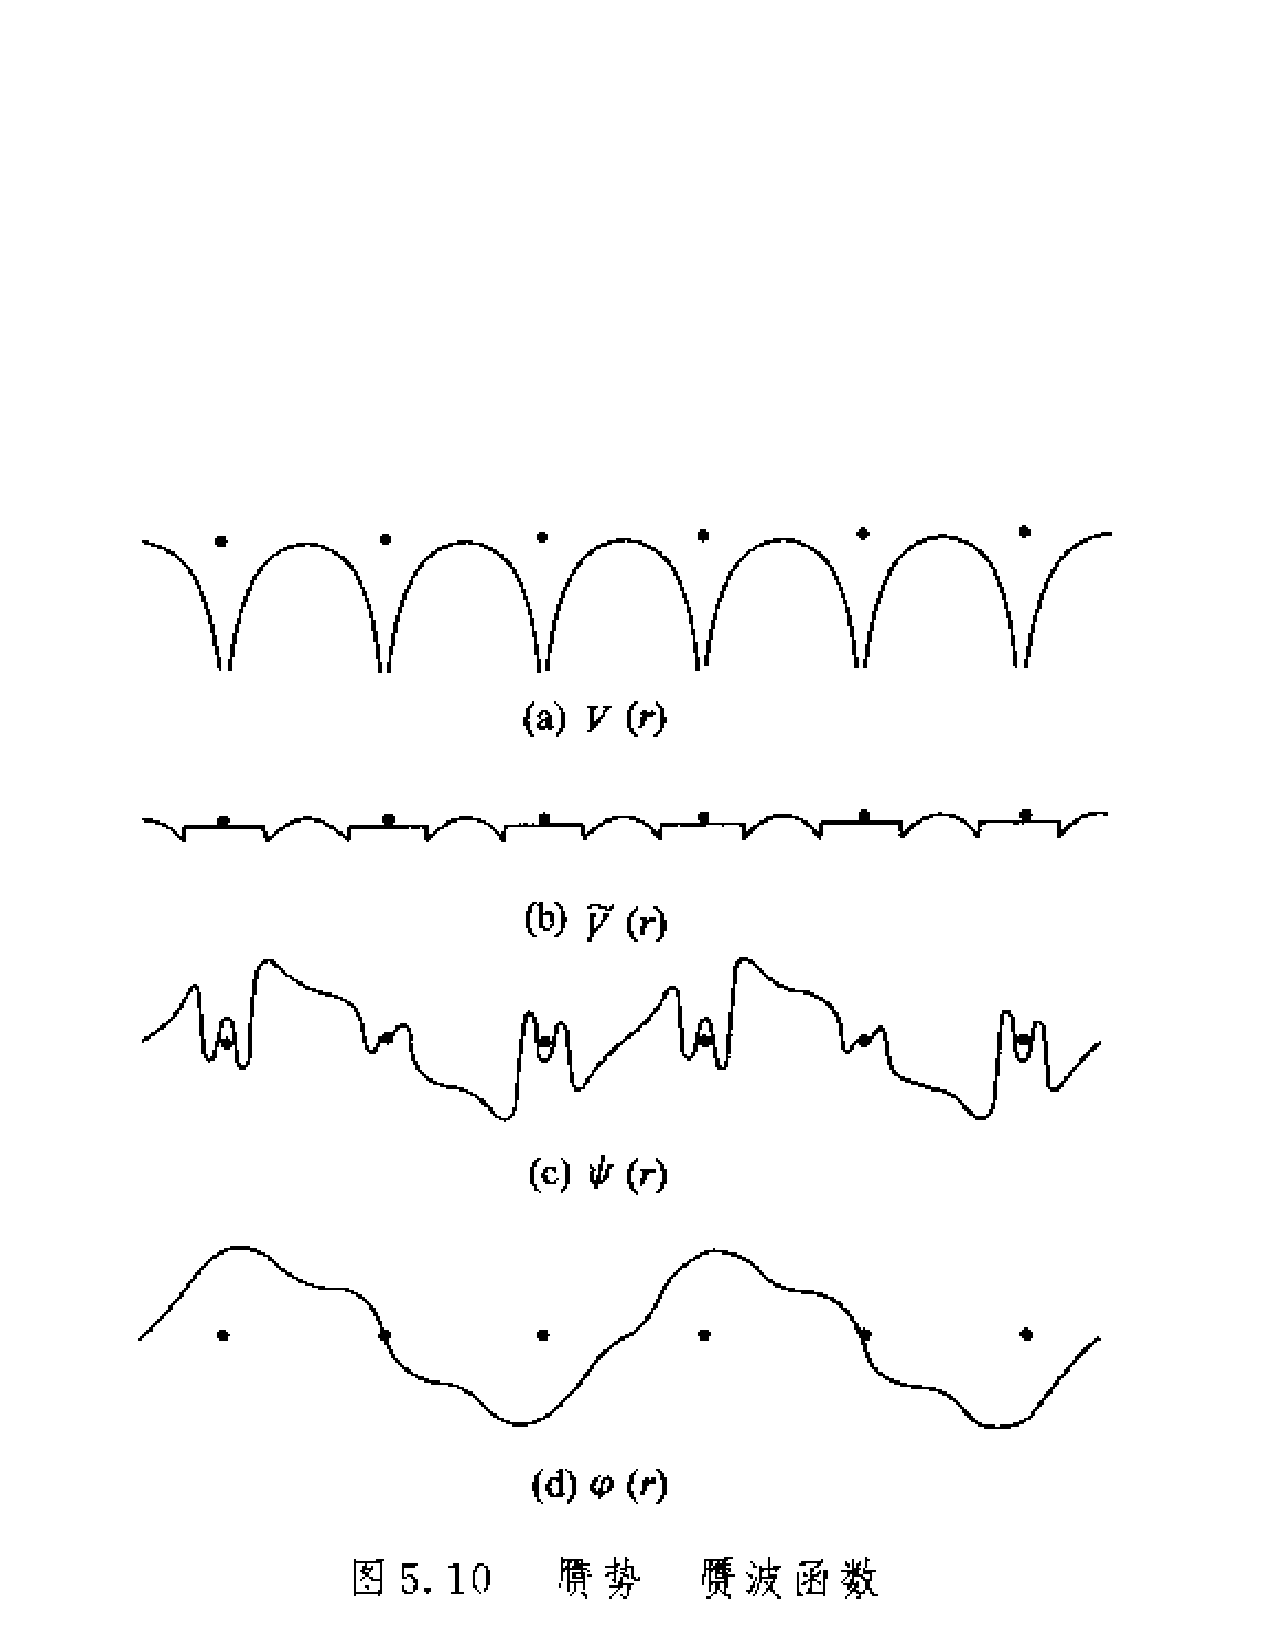
\includegraphics[height=0.8in,width=4.in,viewport=41 433 539 546,clip]{Figures/Pseudo_wave.pdf}\\
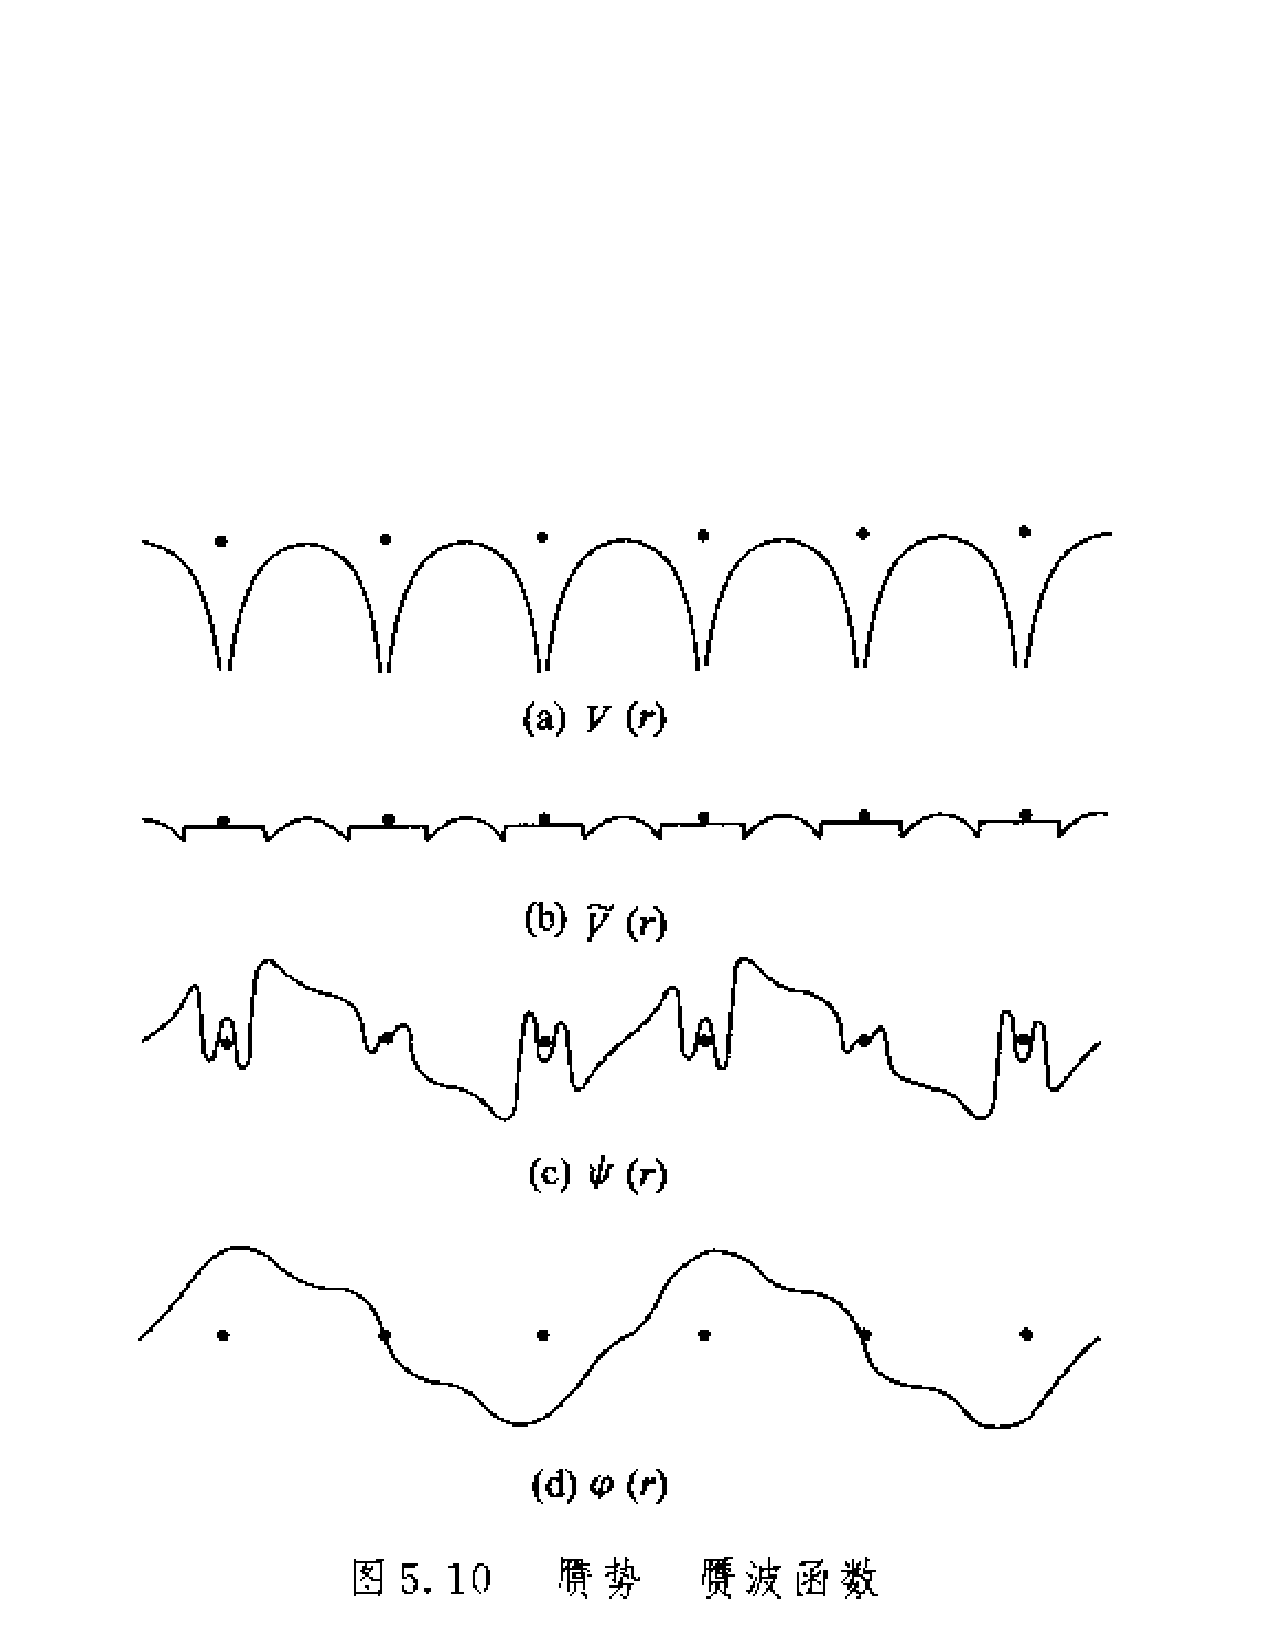
\includegraphics[height=0.8in,width=4.in,viewport=41 210 539 339,clip]{Figures/Pseudo_wave.pdf}
\caption{\small \textrm{The periodic Potential and the wave functions in crystal.}}%(与文献\cite{EPJB33-47_2003}图1对比)
\label{Potential-Wave}
\end{figure}
}

\frame
{
\frametitle{一维自由电子近似微扰}
\begin{figure}[h!]
\centering
%\hspace*{-10pt}
%\vspace*{-1.1in}
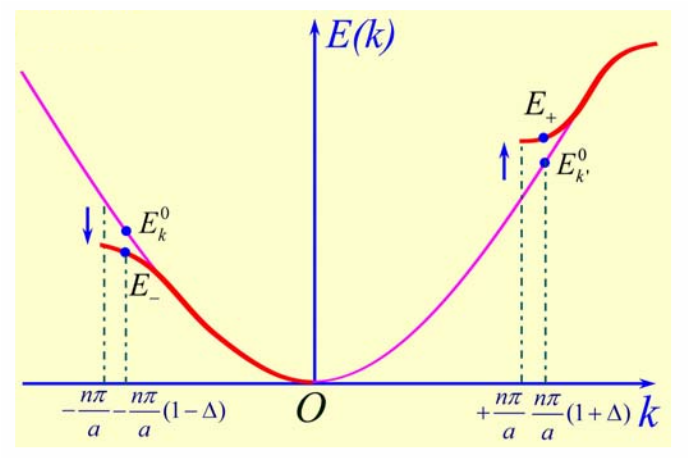
\includegraphics[height=1.5in,width=2.5in,viewport=5 5 700 450,clip]{Figures/Band_Gap-2.png}
%\caption{\small \textrm{The Band-structure from free-electron gas.}}%
\label{Band-Gap-1}
\end{figure} 
\begin{displaymath}
	\begin{aligned}
		&\hat H_0=-\dfrac{\hbar^2}{2m}\dfrac{\mathrm{d}^2}{\mathrm{d}x^2}+\={V} \longrightarrow \hat H=\hat H_0+\hat H^{\prime}=-\dfrac{\hbar^2}{2m}\dfrac{\mathrm{d}^2}{\mathrm{d}x^2}+\={V}+\underline{V(x)-\={V}}\\
		&\Psi_k^0(x)=\dfrac1{\sqrt V}\mathrm{e}^{\mathrm{i}k\cdot x} \longrightarrow \Psi_k(x)=\Psi_k^0(x)+\sum_{k^{\prime}\neq k}\dfrac{\langle k^{\prime}|\hat H^{\prime}|k\rangle}{E_k^0-E_{k^{\prime}}^0}\Psi_{k^{\prime}}^0(x)\\
		&\hat E_k^0=-\dfrac{\hbar^2k^2}{2m}+\={V} \longrightarrow E_k=%E_k^0+E^{\prime}=
		\dfrac{\hbar^2k^2}{2m}+\={V}+\sum_n{}^{\prime}\dfrac{|V_n|^2}{\frac{\hbar^2}{2m}[k^2-(k+2\pi\frac na)^2]}
	\end{aligned}
\end{displaymath}
}

\frame
{
\frametitle{一维自由电子简并微扰}
在波矢$k=\pm\frac{n\pi}{a}$位置,电子能量出现简并态,必须采用简并态微扰理论处理
\begin{figure}[h!]
\centering
%\hspace*{-10pt}
%\vspace*{-1.1in}
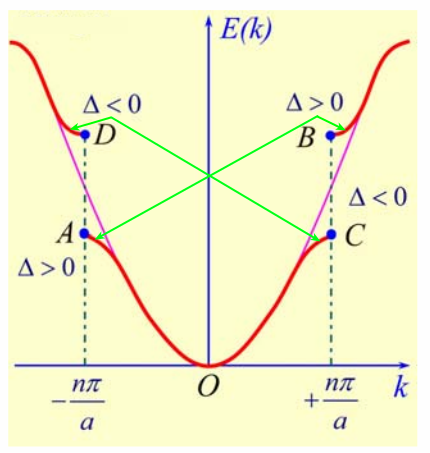
\includegraphics[height=1.3in,width=1.4in,viewport=0 5 420 450,clip]{Figures/Band_Gap-1.png}
%\caption{\small \textrm{The Band-structure from free-electron gas.}}%
\label{Band-Gap-1}
\end{figure} 
\begin{displaymath}
	E_{\textcolor{red}{\pm}}=\left\{
	\begin{aligned}
		&T_n+\={V}\textcolor{red}{+}\Delta^2T_n\bigg(\dfrac{2T_n}{|V_n|}\textcolor{red}{+}1\bigg)\\
		&T_n+\={V}\textcolor{red}{-}\Delta^2T_n\bigg(\dfrac{2T_n}{|V_n|}\textcolor{red}{-}1\bigg)
	\end{aligned}\right.
\end{displaymath}
这里$T_n=\frac{\hbar^2}{2m}\big(\frac{n\pi}a\big)^2$
}

\frame
{
\frametitle{自由电子气模型}
简并态微扰理论引起的能带裂分
\begin{figure}[h!]
\centering
%\hspace*{-10pt}
%\vspace*{-1.1in}
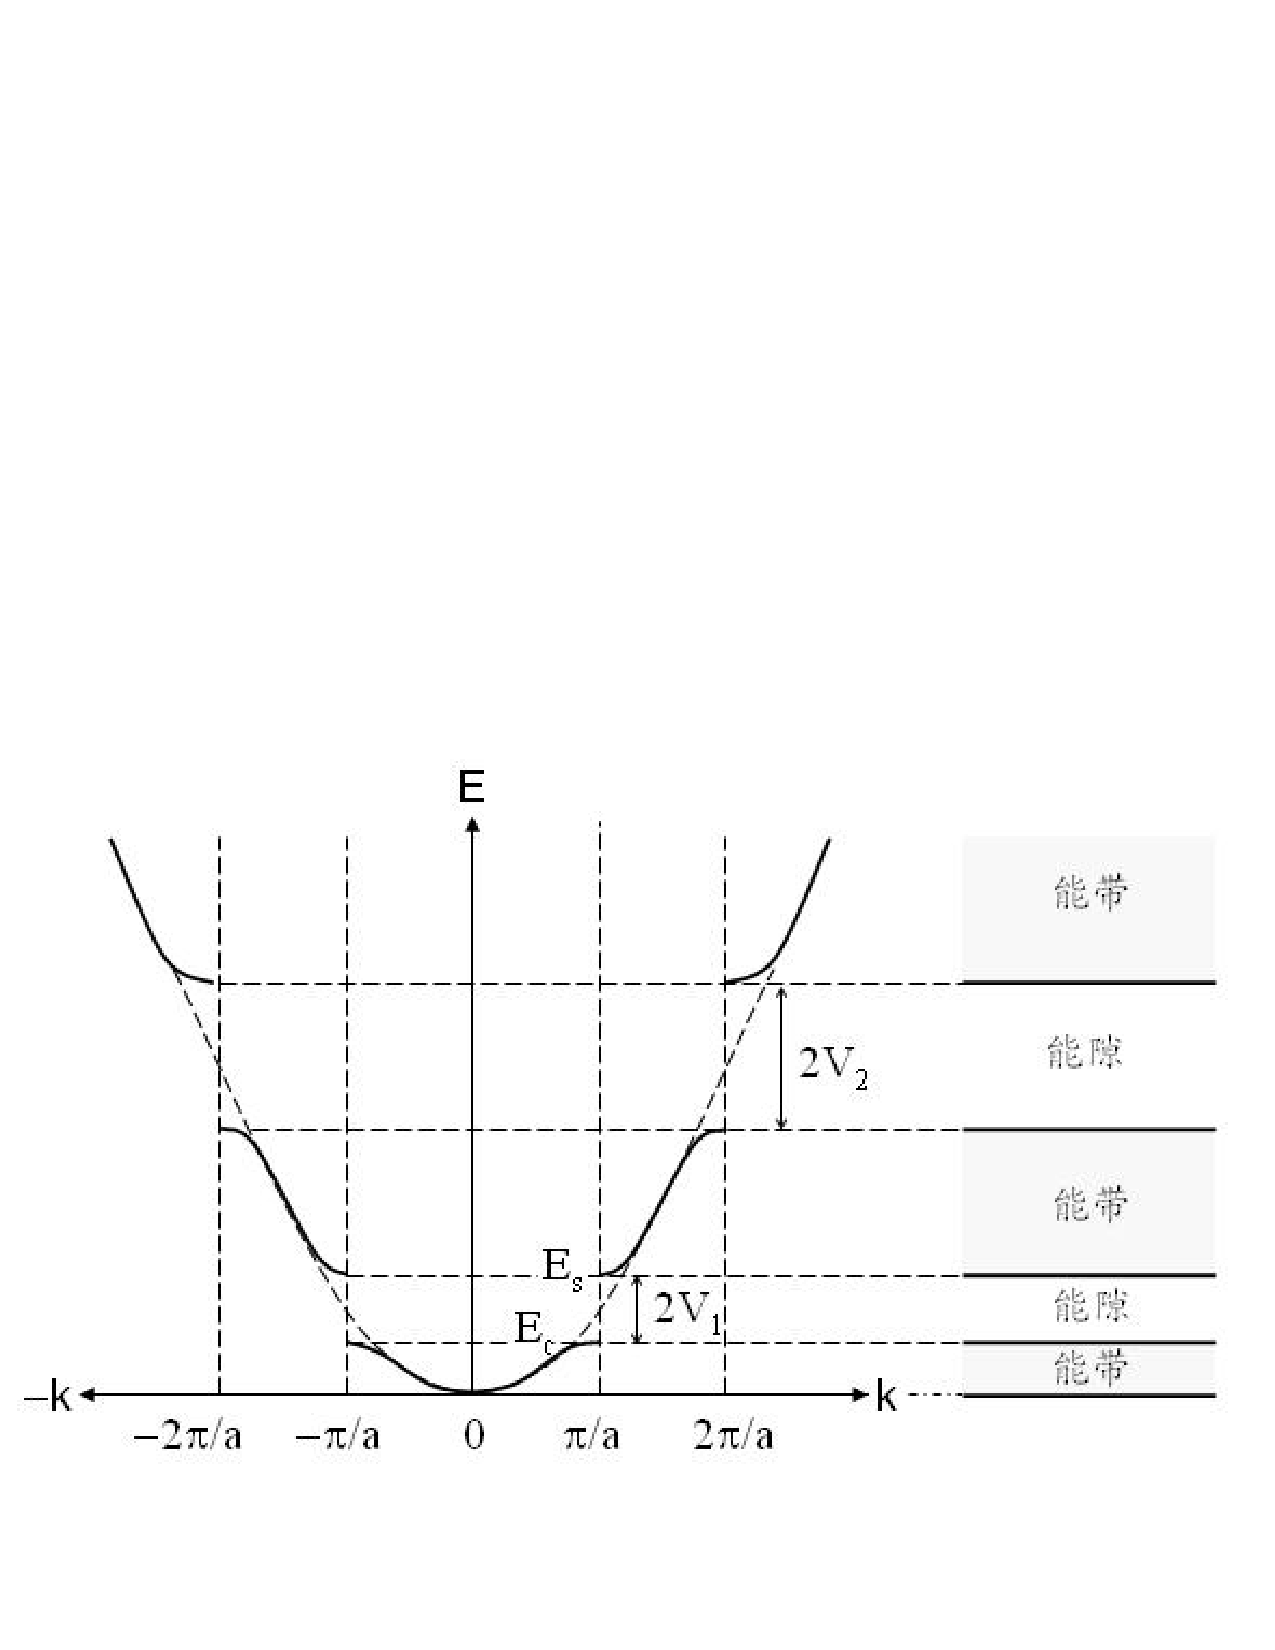
\includegraphics[height=2.1in,width=3.8in,viewport=10 90 570 380,clip]{Figures/Band_Gap.pdf}
\caption{\small \textrm{The Band-structure from free-electron gas.}}%
\label{Band-Structure-1}
\end{figure} 
}

\frame
{
\frametitle{紧束缚模型}
从分子轨道到能带
\begin{figure}[h!]
\centering
\hspace*{-0.29in}
\vspace*{-0.1in}
\subfigure[一维$\mathrm{H}$原子链]{
\label{fig:Hydrogen-1D}
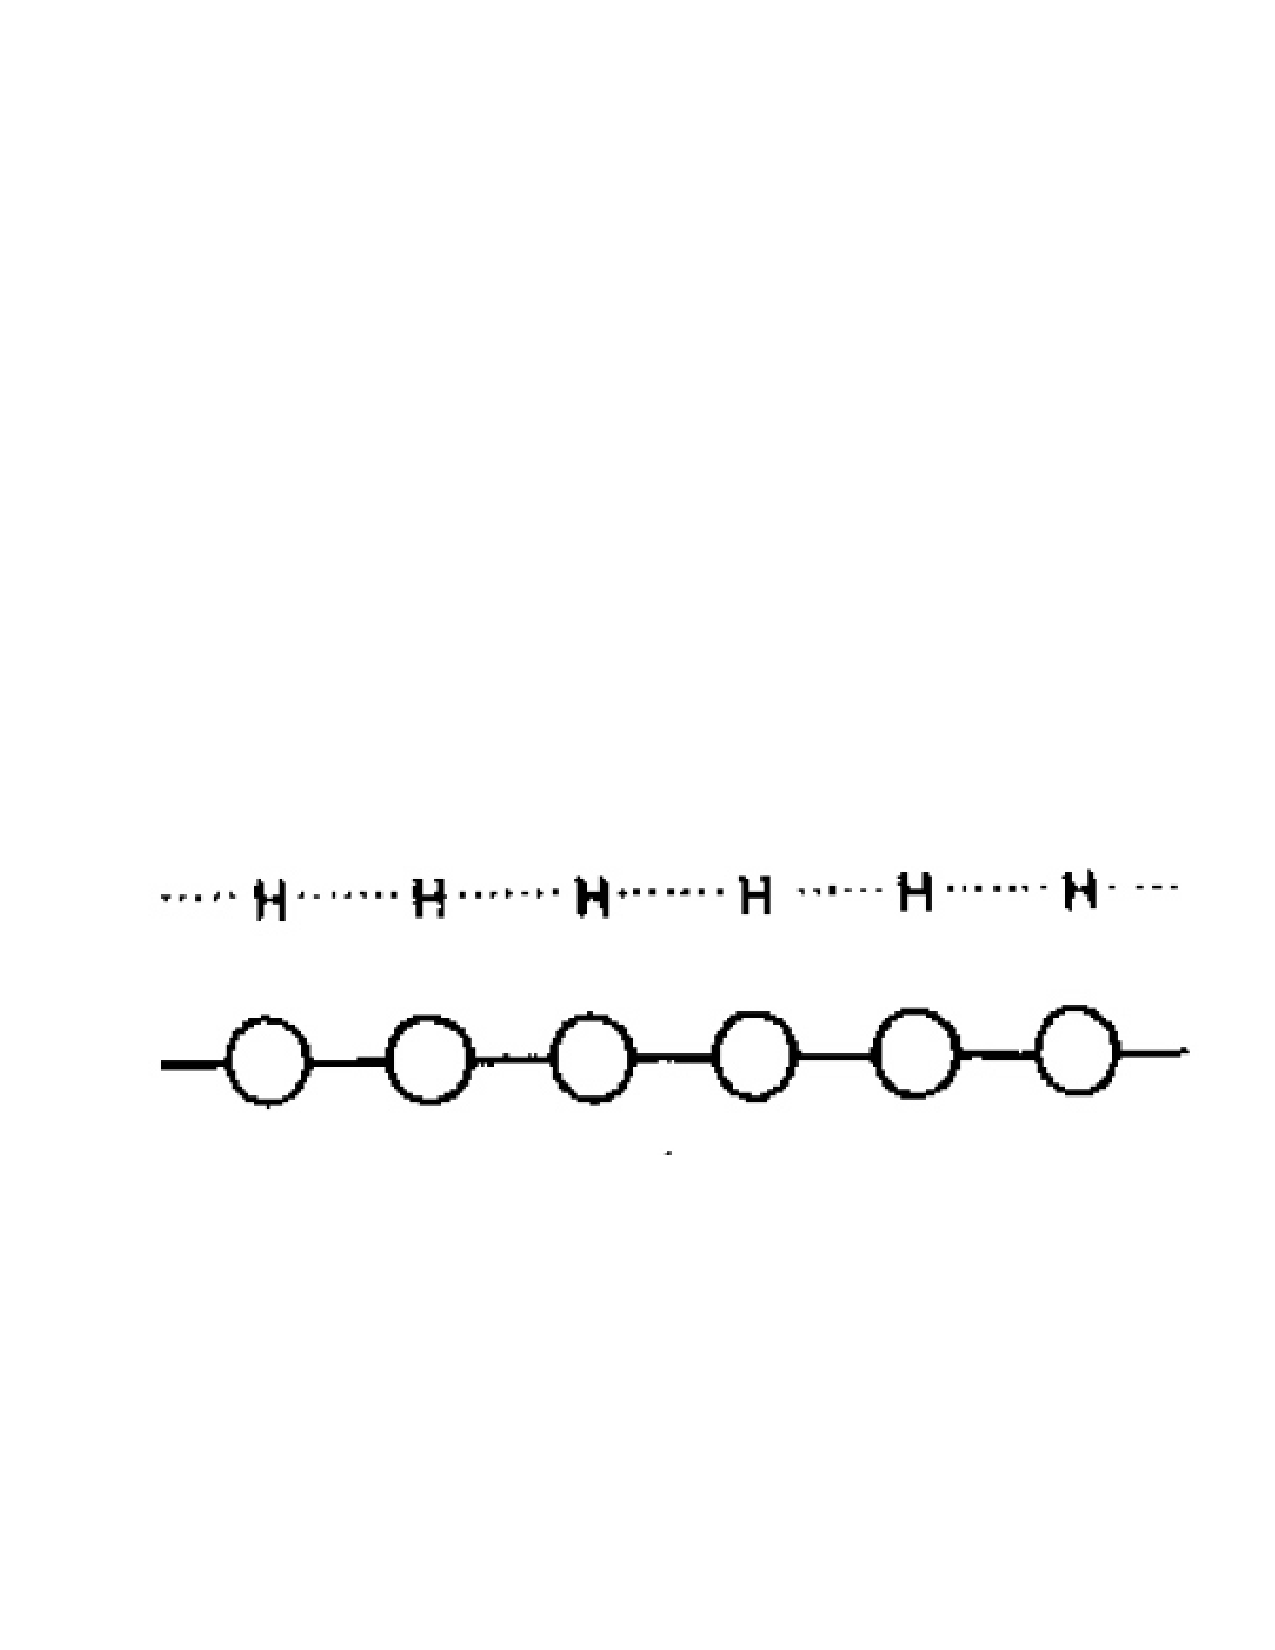
\includegraphics[height=0.25in,width=1.1in,viewport=70 255 570 375,clip]{Figures/Hydrogen-1D.pdf}}
\subfigure[$\mathrm{H}_n$分子轨道]{
\label{fig:Hydrogen-2-n}
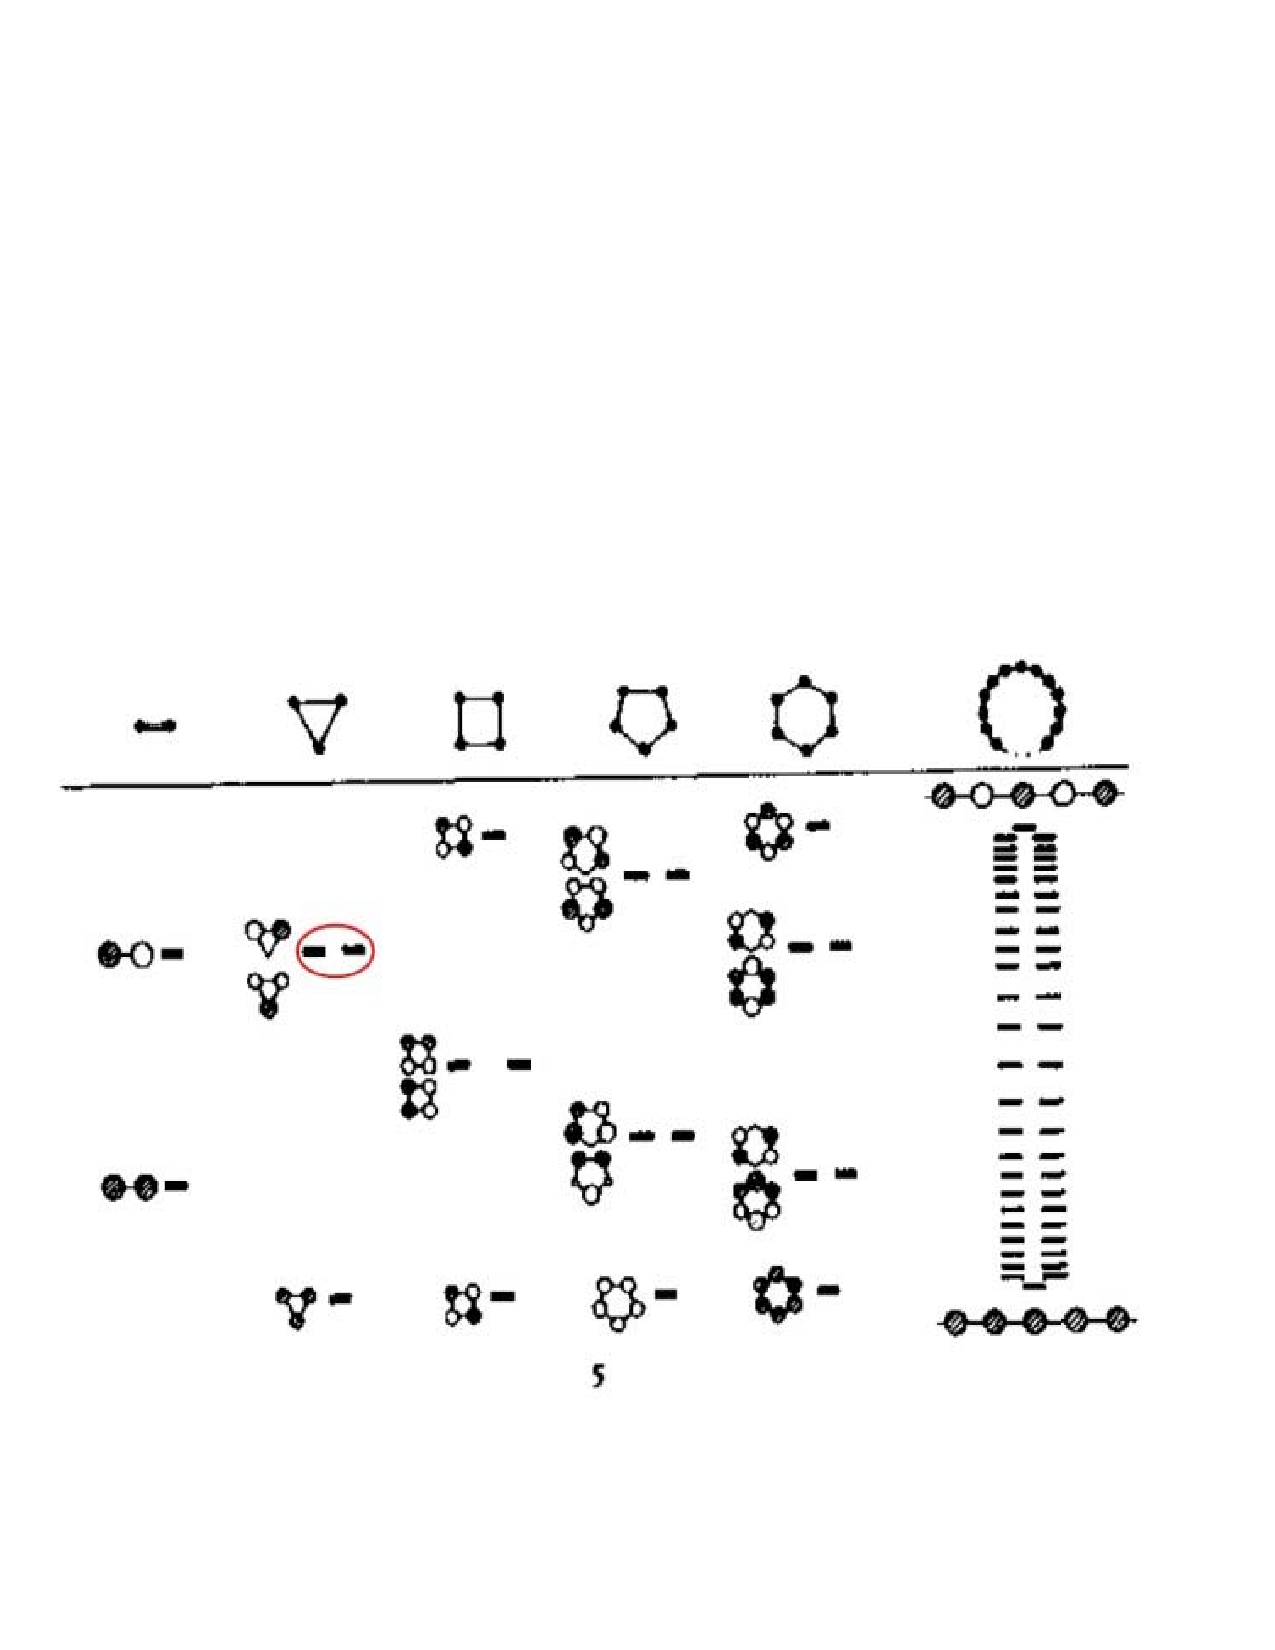
\includegraphics[height=0.8in,width=1.5in,viewport=30 140 545 480,clip]{Figures/Hydrogen-Mol-Orbital.pdf}}
\subfigure[分子波函数]{
\label{fig:Hydrogen-Psi}
\vspace*{-0.2in}
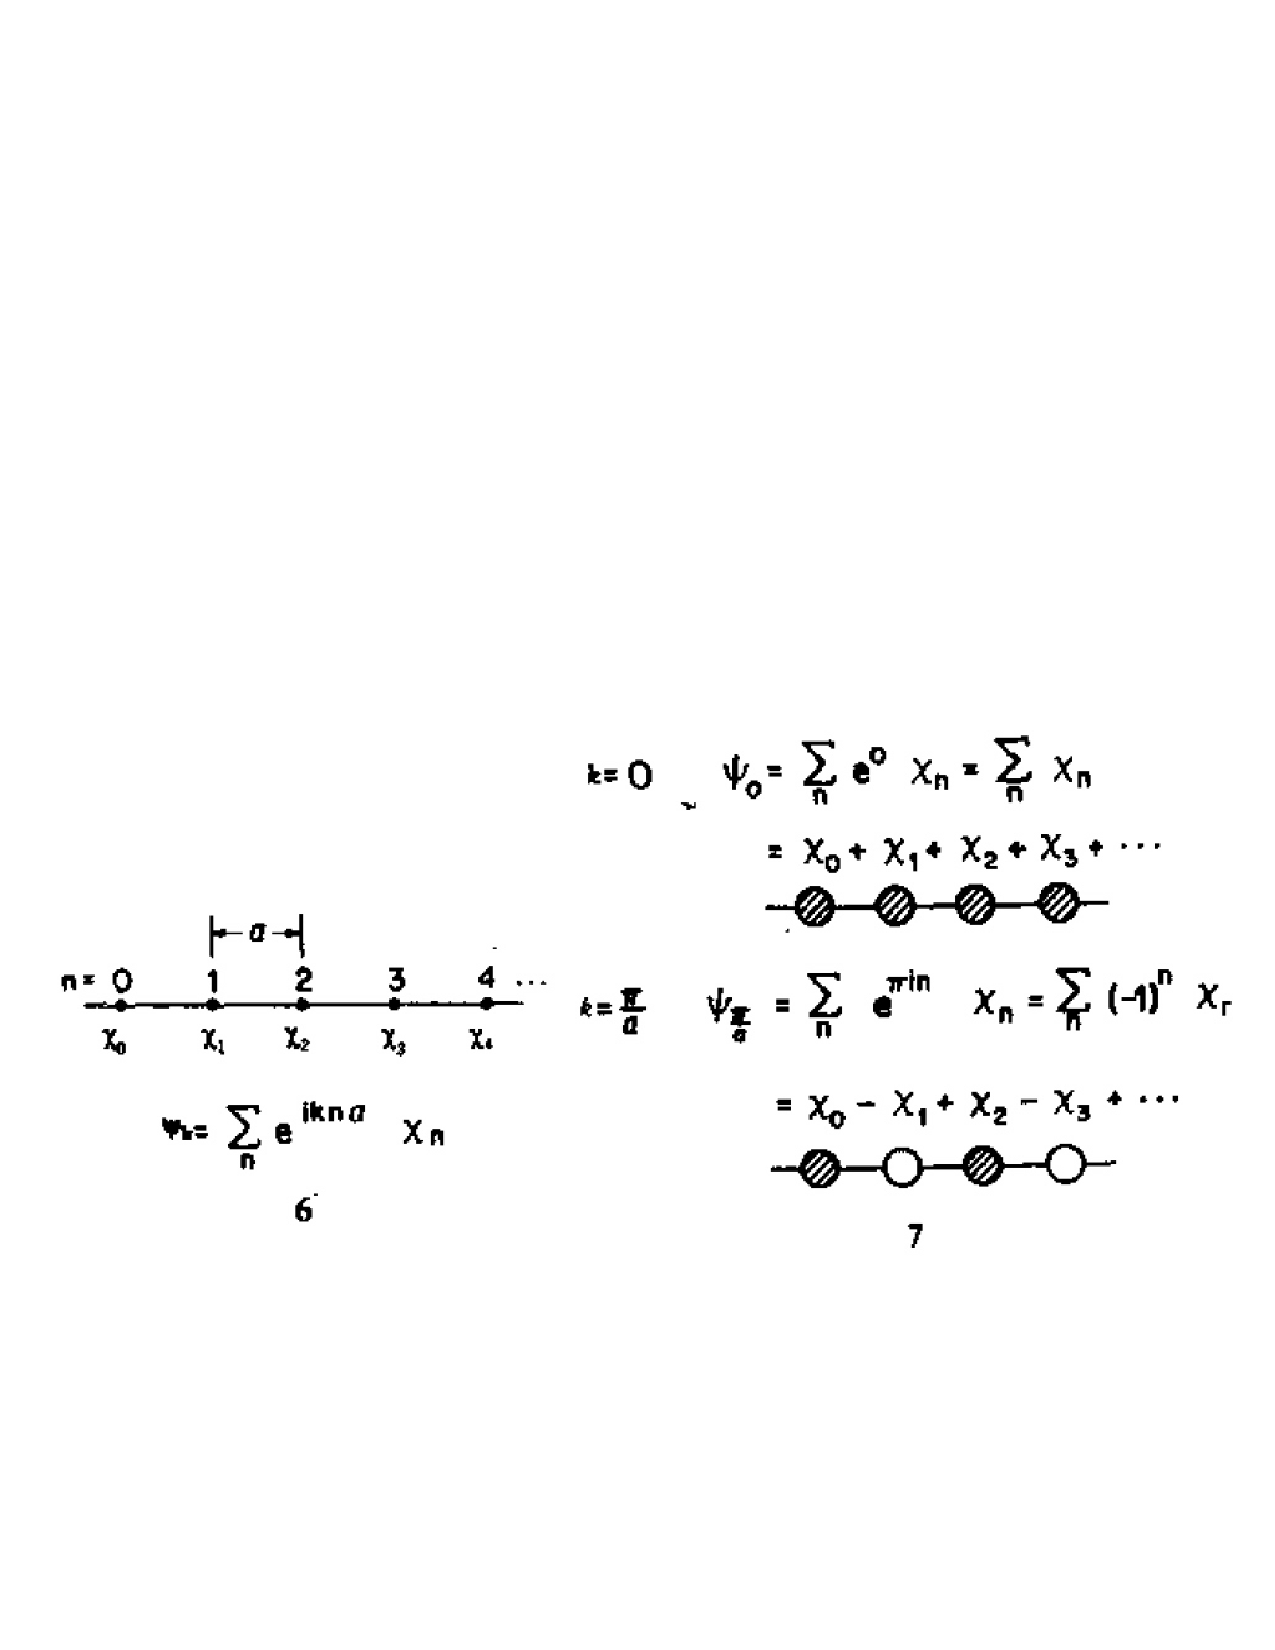
\includegraphics[height=0.5in,width=1.4in,viewport=25 218 595 440,clip]{Figures/Hydrogen-Psi.pdf}}\\
\subfigure[分子轨道与能带]{
\label{fig:Hydrogen-Band-1D}
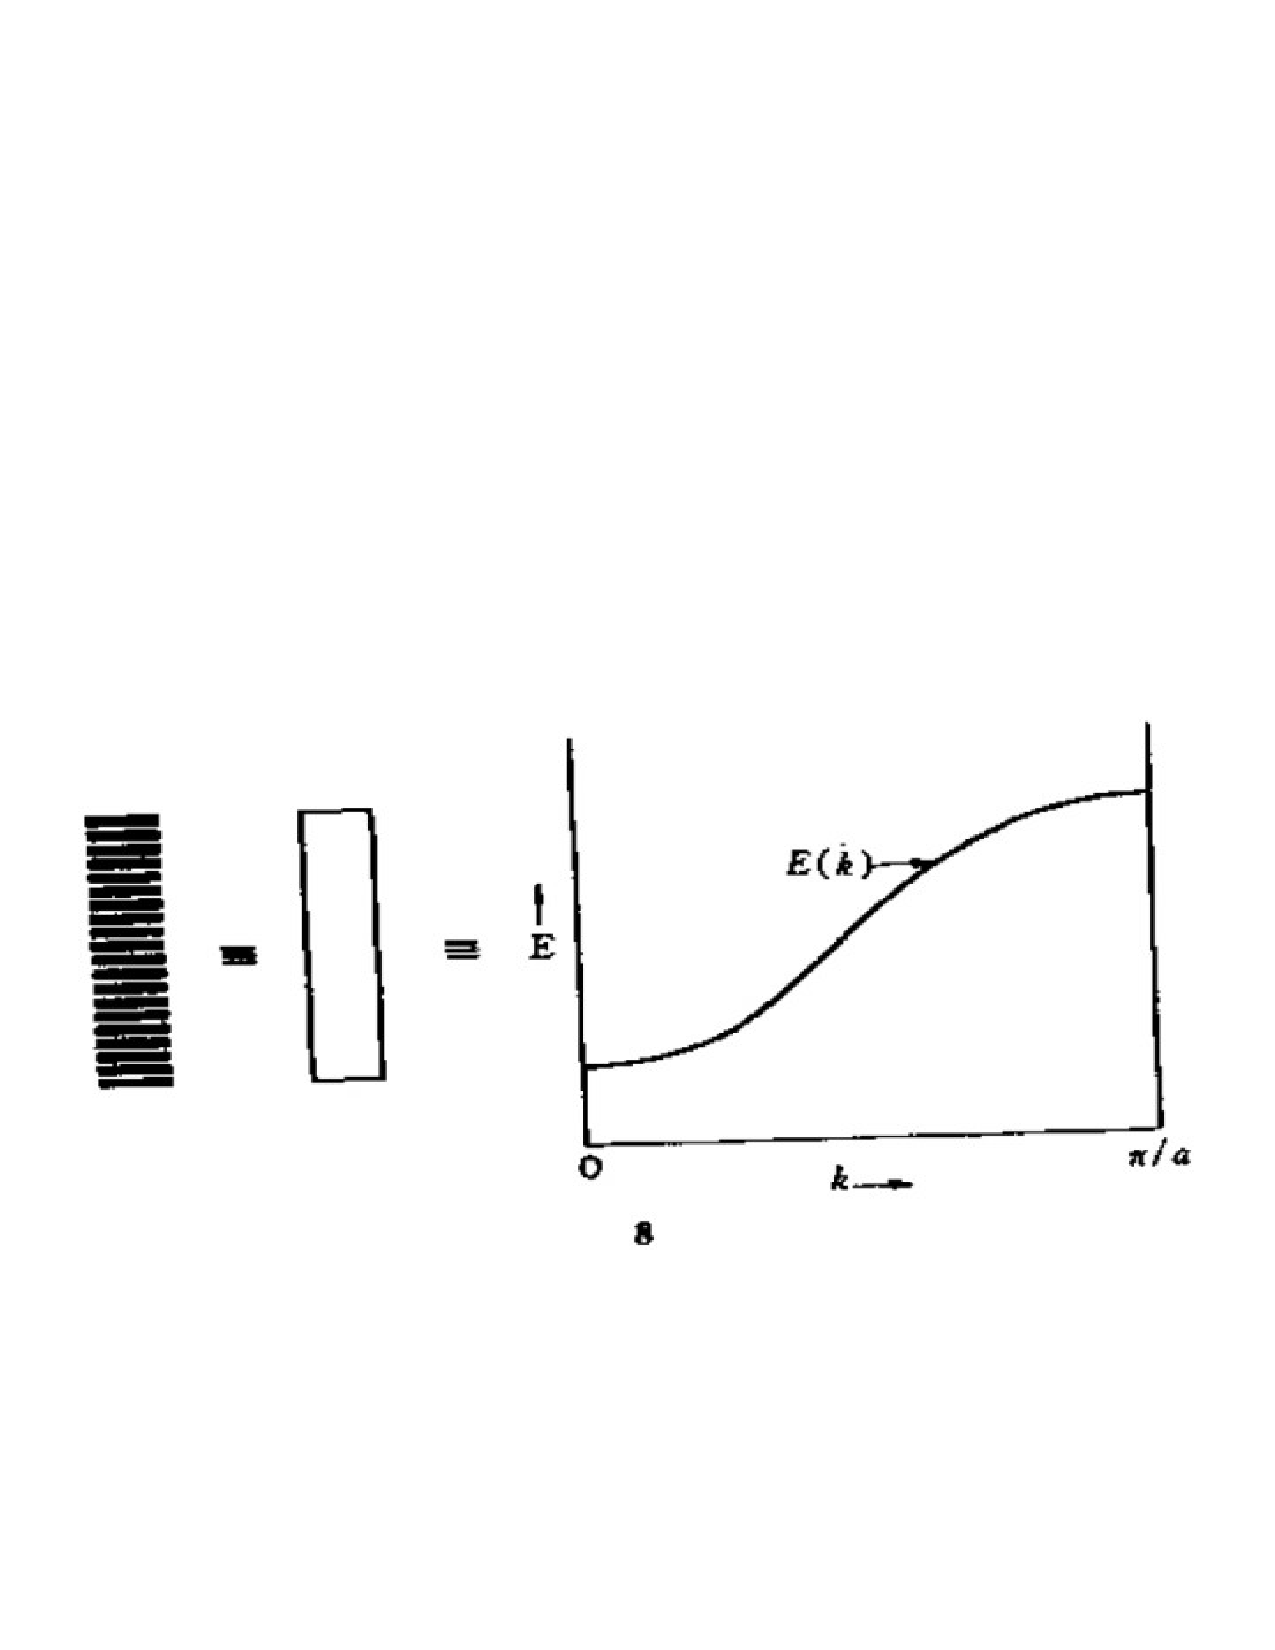
\includegraphics[height=0.6in,width=1.4in,viewport=35 215 575 450,clip]{Figures/Hydrogen-Band-1D.pdf}}
\subfigure[$d$\,轨道]{
\label{fig:Hydrogen-d-Band-1D}
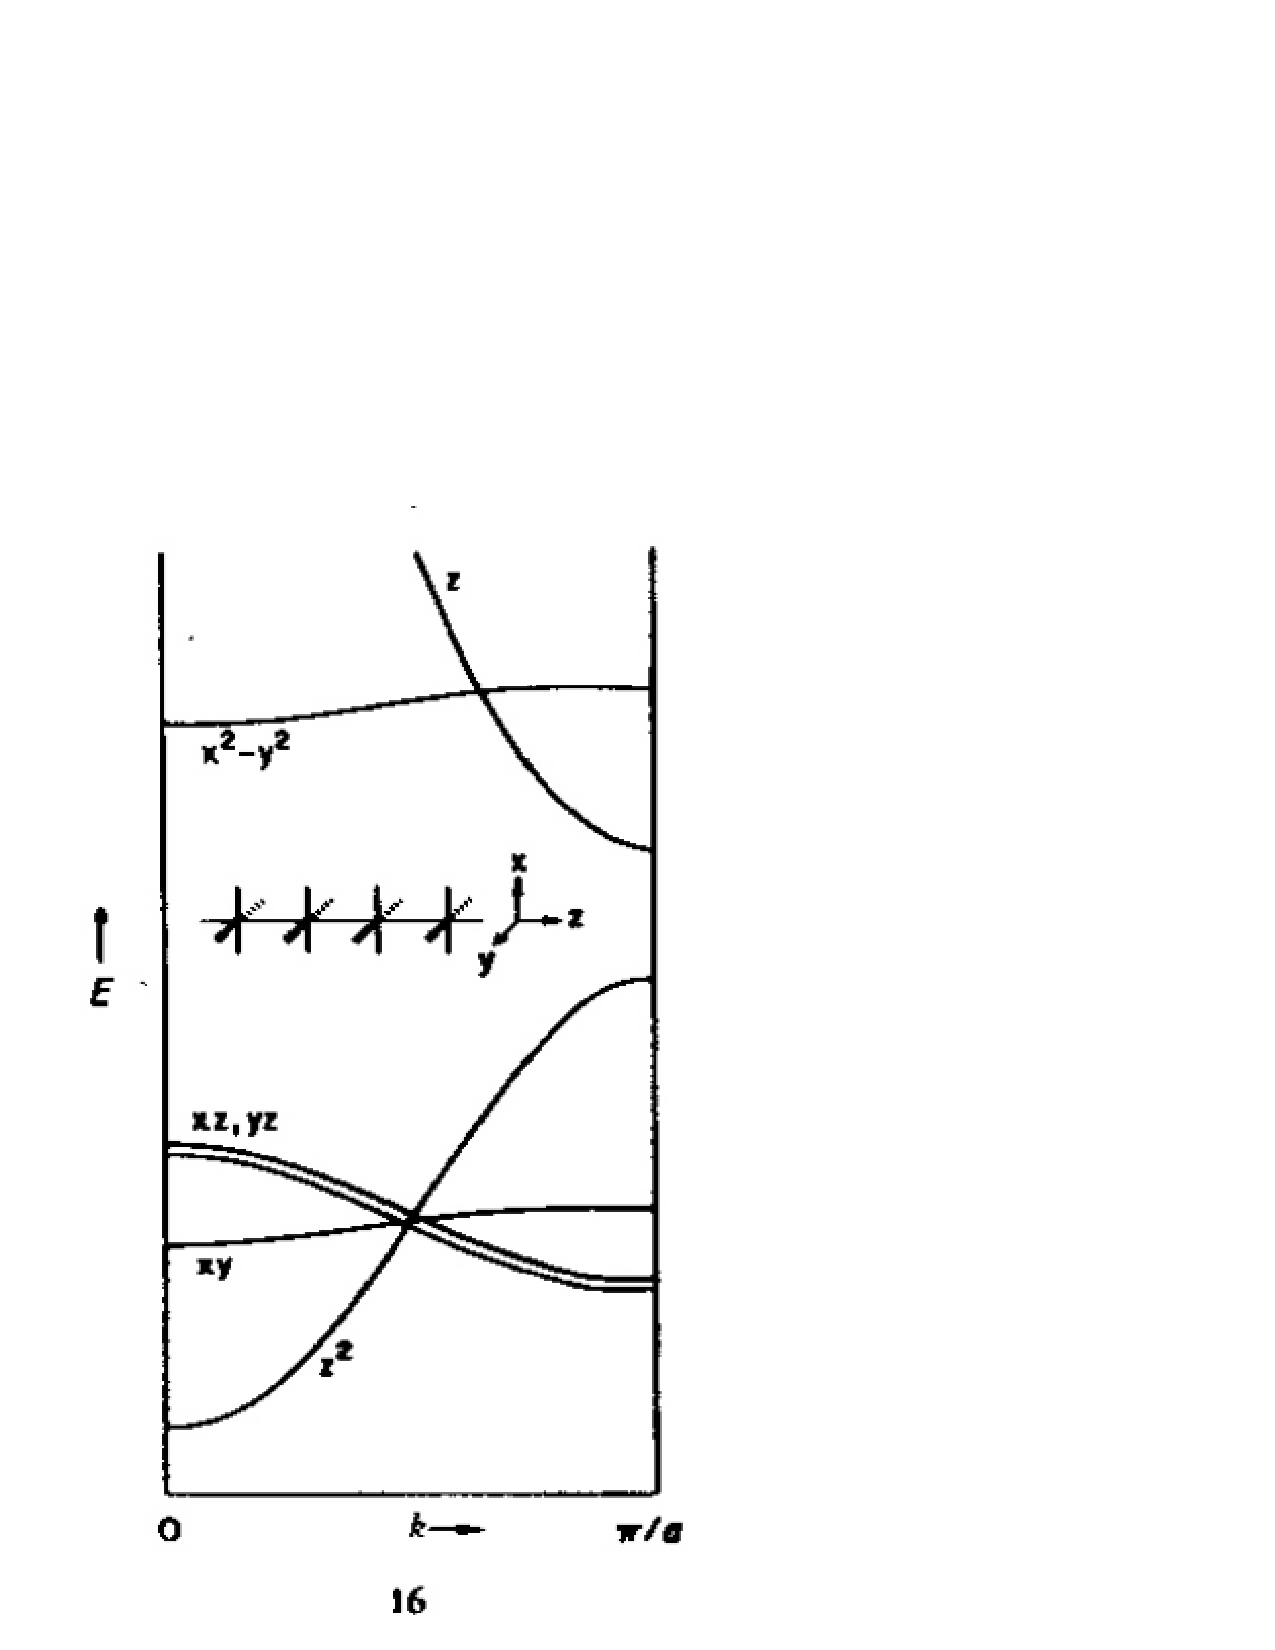
\includegraphics[height=1.0in,width=0.7in,viewport=40 45 330 535,clip]{Figures/Hydrogen-d-Band-1D.pdf}}
\caption{\small \textrm{The Band-structure from Molecular-orbital.}}%
\label{Band-Structure-1}
\end{figure} 
}

\section{能带、k-空间与~Fermi~面}
\frame
{
\frametitle{能带、$\vec k$空间与\textrm{Fermi}面}
\vspace{30pt}
\begin{figure}[h!]
\centering
\hspace*{-0.30in}
\subfigure[\textrm{Band structure}]{
\label{Band_Gap_Fermi-1}
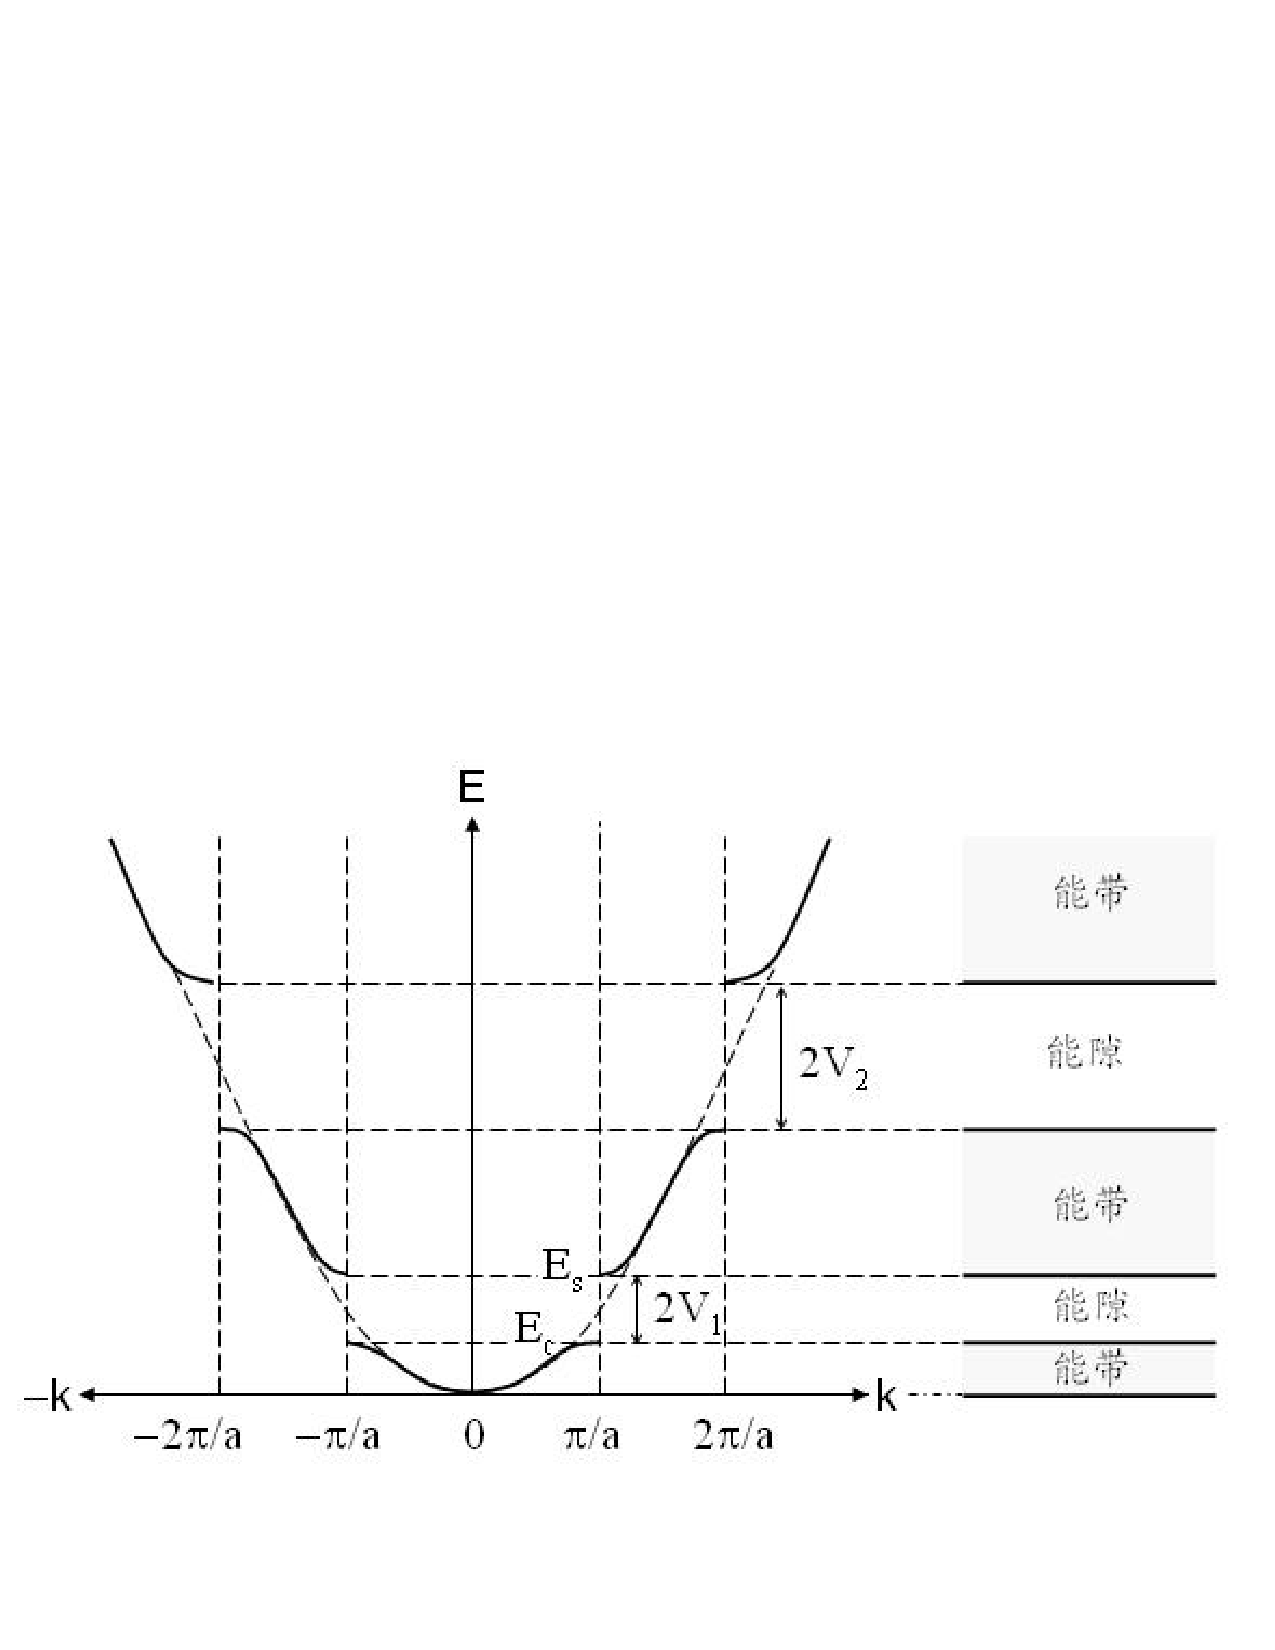
\includegraphics[height=1.3in,width=2.3in,viewport=10 90 570 380,clip]{Figures/Band_Gap.pdf}}
\subfigure[\textrm{Brillouin Zone}]{
\label{Band_Gap_Fermi-2}
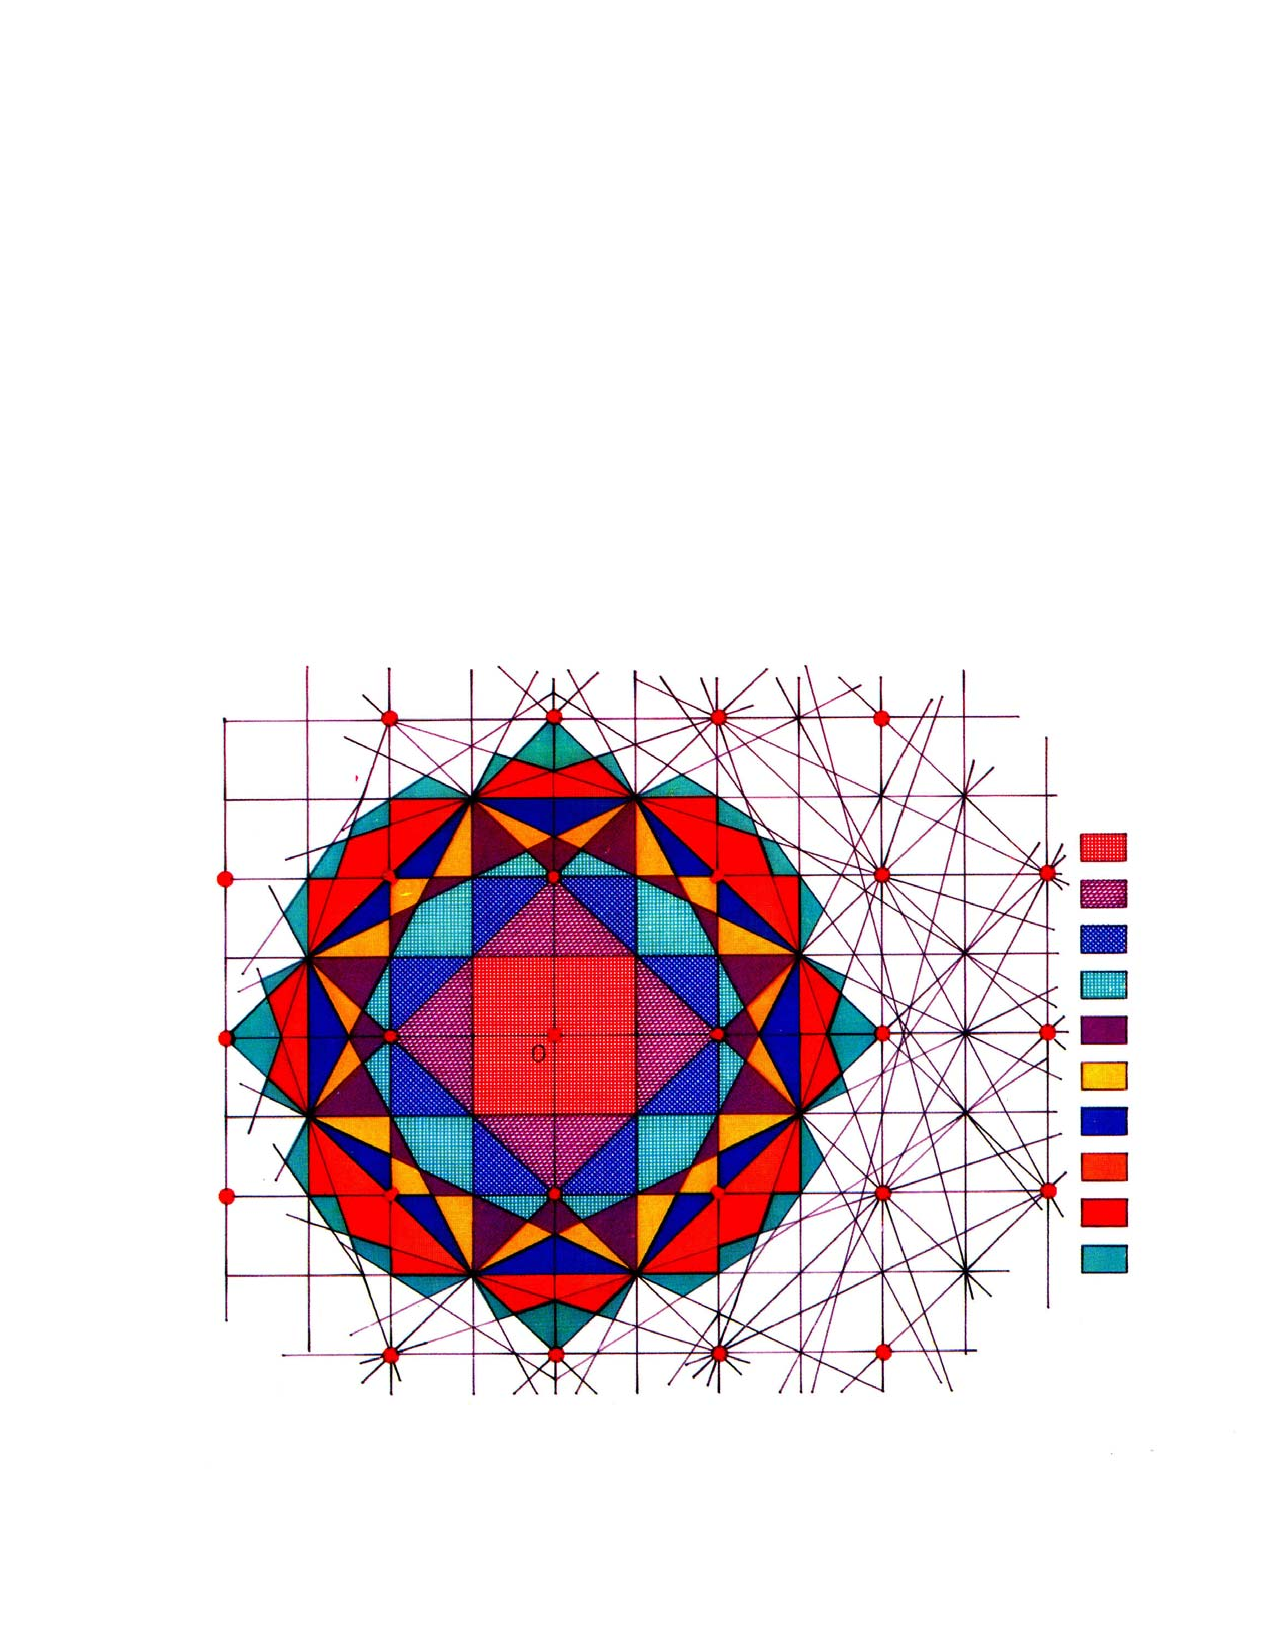
\includegraphics[height=1.28in,width=1.75in,viewport=100 120 545 470,clip]{Figures/2D_Brillouin-Zone.pdf}}
\label{Band_Gap_Fermi}
\end{figure}
}

\frame
{
	\frametitle{简单立方体系的\textrm{Brillouin}区与能带}
\vspace{10pt}
\begin{figure}[h!]
\centering
\hspace*{-0.28in}
\subfigure[\textrm{Brillouin Zone of Cubic lattice}]{
\label{Brillouin_Zone_Cubic}
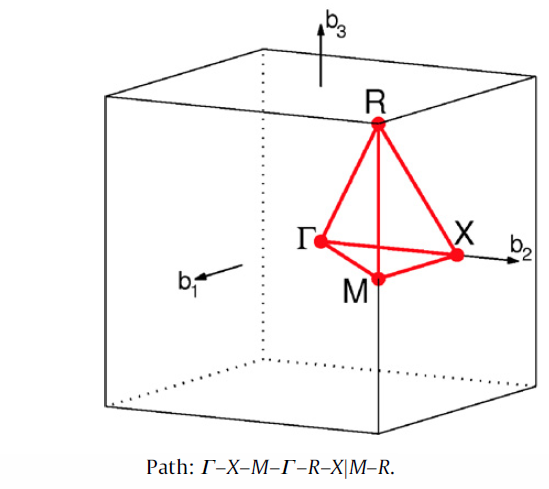
\includegraphics[height=2.1in,width=2.0in,viewport=90 0 550 500,clip]{Figures/Brillouin-Zone_CUB.png}}
\subfigure[\textrm{Band Structure of SrSnO$_3$}]{
\label{Band_Gap_SrSnO3}
\vspace*{-1.00in}
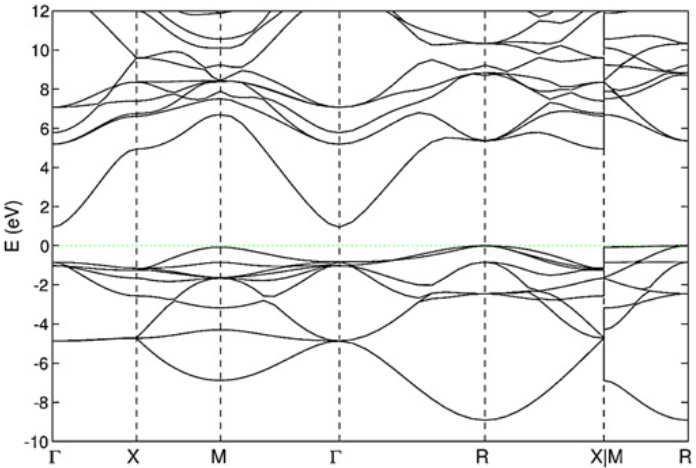
\includegraphics[height=2.10in,width=1.75in,viewport=0 0 710 550,clip]{Figures/Band-Struct_SrSnO3.png}}
\label{Band_Gap_CUB_SrSnO3}
\end{figure}
}

\frame
{
	\frametitle{面心立方体系的\textrm{Brillouin}区与能带}
\vspace{10pt}
\begin{figure}[h!]
\centering
\hspace*{-0.30in}
\subfigure[\textrm{Brillouin Zone of FCC lattice}]{
\label{Brillouin_Zone_FCC}
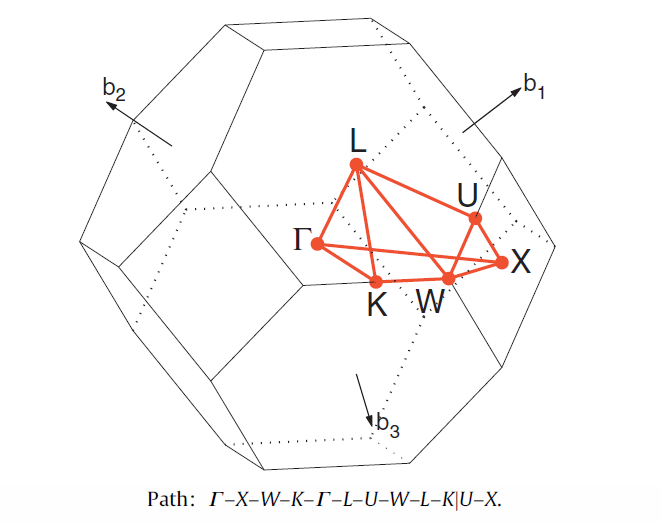
\includegraphics[height=1.9in,width=1.8in,viewport=75 0 560 520,clip]{Figures/Brillouin-Zone_FCC.png}}
\subfigure[\textrm{Band structure of CdS}]{
\label{Band_Gap_CdS}
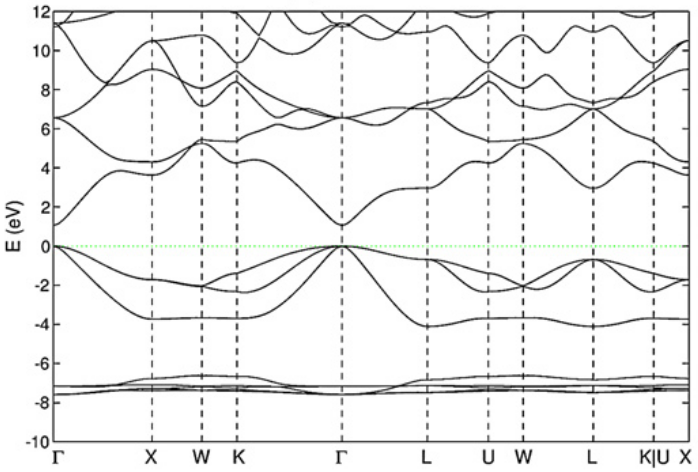
\includegraphics[height=2.10in,width=1.75in,viewport=0 0 580 550,clip]{Figures/Band-Struct_CdS.png}}
\label{Band_Gap_FCC_CdS}
\end{figure}
}

\frame
{
	\frametitle{体心立方体系的\textrm{Brillouin}区与能带}
\vspace{10pt}
\begin{figure}[h!]
\centering
\hspace*{-0.30in}
\subfigure[\textrm{Brillouin Zone of BCC lattice}]{
\label{Brillouin_Zone_BCC}
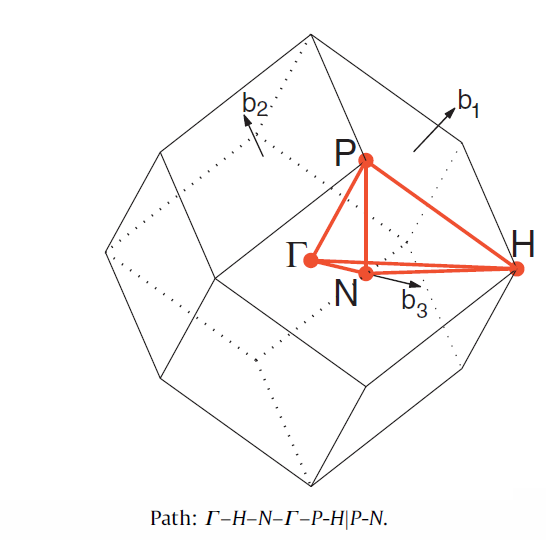
\includegraphics[height=2.1in,width=1.9in,viewport=80 0 550 520,clip]{Figures/Brillouin-Zone_BCC.png}}
\subfigure[\textrm{Band structure of GeF$_4$}]{
\label{Band_Gap_GeF4}
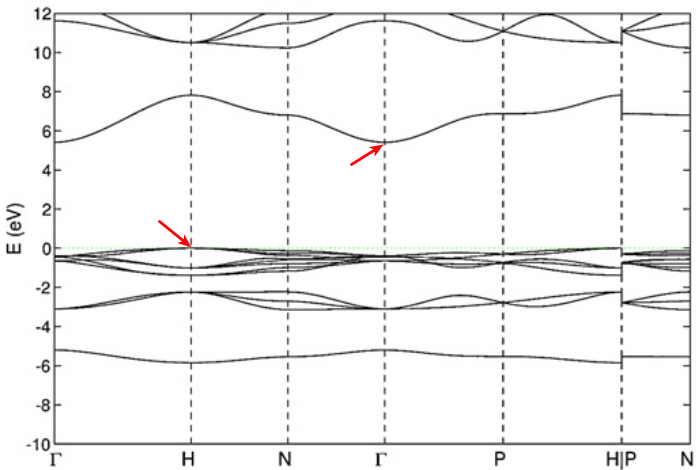
\includegraphics[height=2.10in,width=1.75in,viewport=0 0 580 550,clip]{Figures/Band-Struct_GeF4.png}}
\label{Band_Gap_BCC_GeF4}
\end{figure}
}

\frame
{
%\frametitle{The methods on band structure calculation}
\frametitle{固体能带计算方法}
%\vskip 10pt
%\textrm{The mainly difference of all these methods below: the basis sets and the construction of the potential}
\vskip 10pt
常用的计算方法
\begin{itemize}%[+-| alert@+>]
%\begin{enumerate}%[+-| alert@+>]
\setlength{\itemsep}{12pt}
%  \item \textrm{Plane wave and the pseudo-potential}
	\item	平面波方法
	\item	正交平面波\textrm{(The orthogonalized plane wave, OPW)}和赝势\textrm{(Pseudo-potential, PP)}方法\upcite{Singh_Book,PRB41-7892_1990,JPCM6-8245_1994}
	\item	缀加平面波\textrm{(Augmented plane wave, APW)}方法
	\item	\textrm{MT}轨道\textrm{(Muffin-tin orbitals, MTO)}方法
	\item	投影子缀加波\textrm{(Projector Augmented Wave, PAW)}方法\upcite{PRB50-17953_1994,PRB59-1758_1999}
\end{itemize}
\vskip 5pt 各种方法的\textcolor{red}{主要区别}:~\textcolor{blue}{势函数的处理}与\textcolor{blue}{所选基函数类型}不同
}
%\frame
%{
%\frametitle{发展统一理论框架下的材料计算程序}
%\begin{itemize}
%	\item
%\end{itemize}
%}

\appendix
%------------------------------------------------------------------------Reference----------------------------------------------------------------------------------------------
%\begin{thebibliography}{99}
%-----------------------------------------------------------------------------------------------------------------------------------------------------------------------%
%\frame
%{
%\frametitle{主要参考文献}
%{\small
%\bibitem{Singh_Book}\textrm{D. J. Singh. \textit{Plane Wave, PseudoPotential and the LAPW method} (Kluwer Academic, Boston,USA, 1994)}					%
%  \nocite{*}																				%
%}
%}
%\end{thebibliography}
\begin{thebibliography}{99}
\frame
{
\frametitle{主要参考文献}
{\small
	\bibitem{Huang_Han}黄昆\:原著、韩汝琦\:改编, {\textit{固体物理学}}\:高等教育出版社, 北京, 1988
        \bibitem{Singh_Book}\textrm{D. J. Singh. \textit{Plane Wave, PseudoPotential and the LAPW method} (Kluwer Academic, Boston,USA, 1994)}
        \bibitem{PRB41-7892_1990}\textrm{D. Vanderbilt. \textit{Phys. Rev.} B, \textbf{41} (1990), 7892} 
        \bibitem{JPCM6-8245_1994}\textrm{G. Kresse and J. Hafner. J. Phys: \textit{Condens. Matter}, \textbf{6} (1994), 8245}
        \bibitem{PRB50-17953_1994}\textrm{P. E. Bl\"ochl. \textit{Phys. Rev.} B, \textbf{50} (1994), 17953}
        \bibitem{PRB59-1758_1999}\textrm{G. Kresse and D. Joubert \textit{Phys. Rev.} B, \textbf{59} (1999), 1758}
	\bibitem{Elect_Stru}\textrm{Richard. M. Martin. \textit{Electronic Structure: Basic Theory and Practical Methods} (Cambridge University Press, Cambridge, England, 2004)}
}
\nocite*{}
}
\end{thebibliography}
%{\small
%\phantomsection\addcontentsline{toc}{section}{Bibliography}	 %直接调用\addcontentsline命令可能导致超链指向不准确,一般需要在之前调用一次\phantomsection命令加以修正	%
%\bibliography{Myref}																			%
%\bibliographystyle{mybib}																		%
%  \nocite{*}																				%
%}
%-----------------------------------------------------------------------------------------------------------------------------------------------------------------------%


%-----------------------------------------------------------Beamer下不建议使用bib,因为涉及分页--------------------------------------------------------------------------%
%{\small
%\phantomsection\addcontentsline{toc}{section}{Bibliography}	 %直接调用\addcontentsline命令可能导致超链指向不准确,一般需要在之前调用一次\phantomsection命令加以修正	%
%\bibliography{Myref}																			%
%\bibliographystyle{mybib}																		%
%  \nocite{*}																				%
%}

%------------------------------------------------------------------------------------------------------------------------------------------------------------------------------%

%-------------------------------------------------------------------------Thanks------------------------------------------------------------------------------------------------
%\section{致谢}
%\frame
%{
%\frametitle{致$\quad$谢}
%\begin{itemize}
%    \setlength{\itemsep}{20pt}
%  \item 感谢本团队高兴誉、吴泉生、宋红州等各位老师参与的讨论
%  \item 感谢莫所长、宋主任以及软件中心各位老师和同事
%  \item 感谢王崇愚先生的帮助
%\end{itemize}
%}

\logo{}									%不显示logo
\frame
{
\vskip 60 pt
%\hskip 10pt \textcolor{blue}{\Huge 感谢答辩委员会各位老师\,\textrm{!}}\\
\vskip 35 pt
\hskip 60pt \textcolor{blue}{\Huge 谢谢大家\:!}
%\vskip 15 pt
%\hskip 40pt \textcolor{blue}{\Huge \textrm{for your attention\:!}}
}

%-------------------------------------------------------------------------------------------------------------------------------------------------------------------------------

\clearpage
%\end{CJK*}
\end{document}
